\section{First Increment Production - Acceptance tests report}
The tests that have been done are validating the software, that's to say it tests all the platform with a complete simulation, form the
input of data to the output of the results, doing computations.

\subsection{Report on the bouncing ball example}
The acceptance test has been run, the file \ref{BouncingBall_TIDS.xml} has been read and computations has been done to make a ball
bouncing on a rigid plan. On the \ref{acceptanceTest} we can see the position of the ball, the velocity of this ball
and the force that make the ball bouncing when it touch the floor.

\subsubsection{Results of the bouncing ball test}
\begin{figure}[!hbp]
\begin{center}
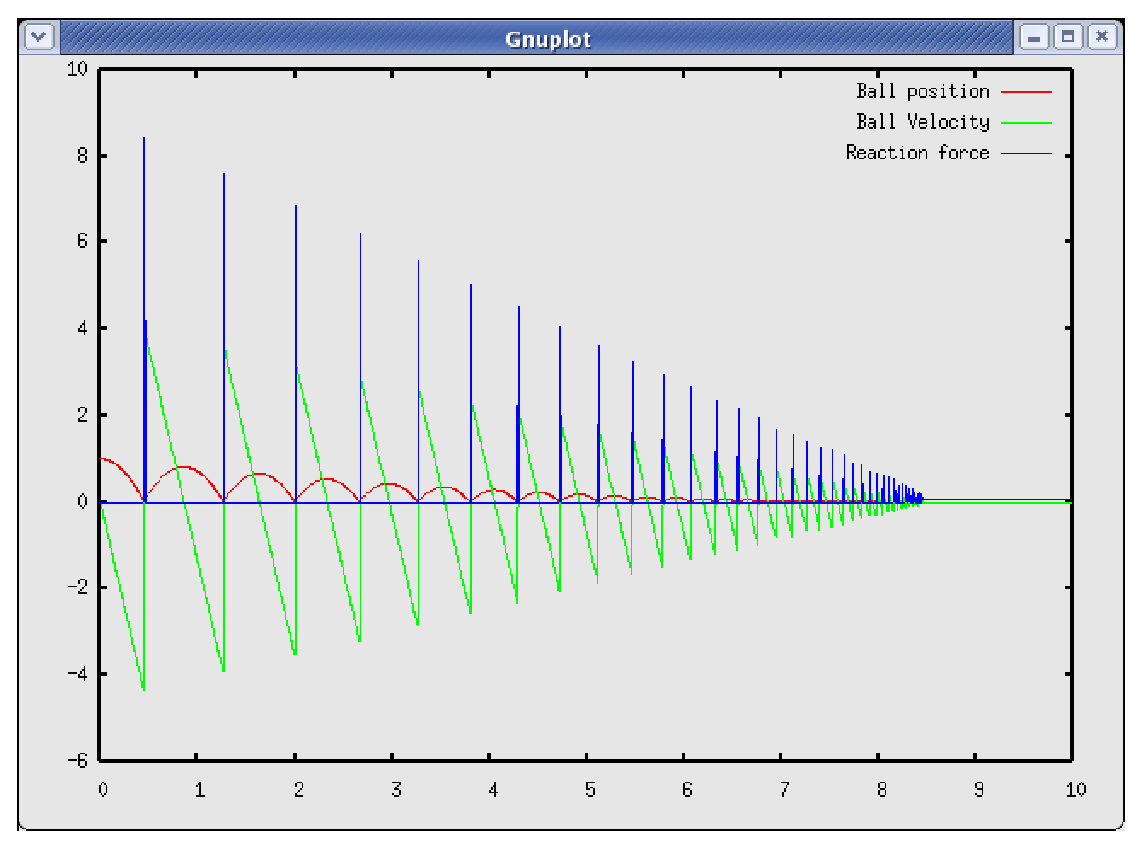
\includegraphics[scale=0.80]{figure/acceptanceTest.ps}
\caption{The bouncing ball}
\label{acceptanceTest}
\end{center}
\end{figure}

\subsubsection{\ac{xml} input file of the bouncing ball test}
\label{BouncingBall_TIDS.xml}
\verbatiminput{BouncingBall_TIDS.xml}
